\documentclass{standalone}
\usepackage{tikz}

\begin{document}
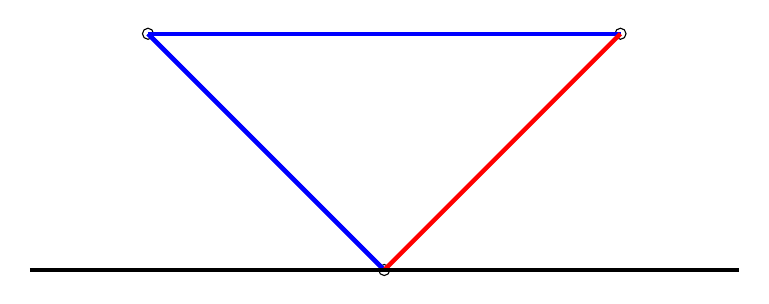
\begin{tikzpicture}[scale=1.5]

% Define node styles
\tikzset{
    vertex/.style={circle, draw, fill=white, minimum size=4pt, inner sep=0},
}

% Define coordinates for the nodes
\coordinate (A) at (0,2); % Top-left node
\coordinate (B) at (4,2); % Top-right node
\coordinate (C) at (2,0); % Bottom-center node

% Draw the nodes
\node[vertex] at (A) {};
\node[vertex] at (B) {};
\node[vertex] at (C) {};

% Draw the edges
\draw[ultra thick, blue] (A) -- (B); % Blue horizontal edge
\draw[ultra thick, blue] (A) -- (C); % Blue diagonal edge (left)
\draw[ultra thick, blue] (A) -- (C); % Redundant drawing for clarity
\draw[ultra thick, red] (B) -- (C); % Red diagonal edge (right)

% Draw the ground line
\draw[ultra thick, black] (-1,0) -- (5,0);

\end{tikzpicture}
\end{document}